\section{Software Aspects}

\subsection{Display Stack Overview}

\begin{frame}{System-agnostic overview: kernel}
  \begin{itemize}
  \item The kernel provides access to the hardware from userspace
  \item Handles clocks, power, register access, interrupts, etc
  \item Coordinates memory management with the rest of the system
  \item Exposes features to userspace through hardware-agnostic interfaces\\
  \textit{or at least, as much as possible}
  \item Three aspects are usually involved:
    \begin{itemize}
    \item \textbf{display}: from framebuffer to encoder
    \item \textbf{render}: GPU and/or 2D accelerators
    \item \textbf{input}: keyboard, mouse and other devices
    \end{itemize}
  \end{itemize}
\end{frame}

\begin{frame}{System-agnostic overview: display userspace}
  \begin{itemize}
  \item The kernel provides \textbf{exclusive access} to display hardware
  \item Many applications need to show their buffers concurrently
  \item The \textbf{display server} is in charge of coordinating between applications:
    \begin{itemize}
    \item Part of the core of the system, privileged
    \item Applications (via libraries) contact the server to display pixel buffers
    \item Dispatches input events to the concerned applications
    \item Only the display server deals with the kernel display and input APIs
    \end{itemize}
  \item The \textbf{compositor} merges pixel buffers from applications into the final buffer
  \item The \textbf{window manager} defines stacking order, focus, decorations, etc
  \item Both can be part of the display server or distinct components
  \item Serious security concerns: I/O isolation for applications, server privileges
  \end{itemize}
\end{frame}

\begin{frame}{System-agnostic overview: display userspace (illustrated)}

  \begin{minipage}[t]{0.49\textwidth}
    \centering
    \includegraphics[height=7em]{slides/graphics-software/compositing-gnome-shell.jpg}\\
    \textit{\small GNOME-Shell (green) displaying the\\ top-bar and background}\\
    \vspace{0.5em}
    \includegraphics[height=7em]{slides/graphics-software/compositing-gnome-terminal.jpg}\\
    \textit{\small GNOME-Terminal (green) with\\ window decorations (red)}
  \end{minipage}
  \hfill
  \begin{minipage}[t]{0.49\textwidth}
    \centering
    \includegraphics[height=7em]{slides/graphics-software/compositing-lollipop.jpg}\\
    \textit{\small Lollipop (green) with\\ window decorations (red)}\\
    \vspace{0.5em}
    \includegraphics[height=7em]{slides/graphics-software/compositing-result.jpg}\\
    \textit{\small The composited result}
  \end{minipage}
\end{frame}

\begin{frame}{System-agnostic overview: render userspace}
  \begin{itemize}
  \item Graphics applications and libraries need to render visual elements
  \item Rendering can be a major \textbf{performance bottleneck}
  \item The system often provides \textbf{accelerated 2D primitives}:
    \begin{itemize}
    \item Either in the display server
    \item Either in dedicated libraries
    \end{itemize}
  \item Their implementation can take different forms:
    \begin{itemize}
    \item Using dedicated 2D hardware
    \item Using 3D hardware in 2D setups (\(z = 0\))
    \item Using specific efficient CPU instructions (SIMD)
    \item Using optimized generic algorithms
    \end{itemize}
  \item \textbf{3D rendering} comes with its own interfaces and libraries
  \item Usually with generic interfaces and hardware-specific implementations
  \end{itemize}
\end{frame}

\begin{frame}{System-agnostic overview (illustrated)}
  \begin{center}
  \includegraphics[width=\textwidth]{slides/graphics-software/agnostic-display-stack-overview.pdf}
  \end{center}
\end{frame}

\begin{frame}{Linux kernel overview}
  \begin{itemize}
  \item \textbf{Input} subsystem
    \begin{itemize}
    \item Supports devices such as mice, keyboards, joysticks, touchscreens
    \item Legacy (unused) interfaces for keyboard, mice
    \item Unified \textbf{evdev} event interface to simplify userspace
    \end{itemize}
  \item \textbf{Framebuffer device} (fbdev) subsystem
    \begin{itemize}
    \item \textbf{Legacy} interface for displaying pixel buffers on-screen
    \item Very limited pipeline configuration, no hotplug support
    \item Extended features added through driver-specific interfaces
    \end{itemize}
  \item \textbf{Direct Rendering Manager} (DRM) subsystem
    \begin{itemize}
    \item Unified display configuration interface: \textbf{Kernel Mode Setting} (KMS or DRM mode)
    \item Allows synchronizing changes together (DRM atomic)
    \item Exposes render devices through driver-specific interfaces (DRM render)\\
      \textit{Mostly for 3D rendering with GPUs, but a few 2D devices too}
    \item Provides memory management mechanisms (DRM GEM)
    \end{itemize}
  \end{itemize}
\end{frame}

\begin{frame}{Linux-compatible low-level userspace overview}
  \begin{itemize}
  \item \textbf{Input} low-level libraries
    \begin{itemize}
    \item \textbf{libevdev} (C): Wrapper for evdev interface system calls
    \item \textbf{libinput} (C): Input device management, abstraction and quirks, using libevdev
    \end{itemize}
  \item \textbf{Display/render} low-level interface library
    \begin{itemize}
    \item \textbf{libdrm} (C): Wrapper for DRM system calls
    \end{itemize}
  \item \textbf{2D render} low-level libraries
    \begin{itemize}
    \item \textbf{Pixman} (C): Optimized pixel-level operations
    \item \textbf{Cairo} (C): Optimized vector drawing (can use 3D)
    \item \textbf{Skia} (C): Optimized vector drawing from Google (can use 3D)
    \item \textbf{Clutter} (C++): Accelerated UI animation (using 3D)
    \end{itemize}
  \item \textbf{3D render} low-level libraries
    \begin{itemize}
    \item \textbf{Mesa 3D} (C): Reference free software OpenGL implementation
    \item \textbf{Proprietary vendor implementations} for specific hardware
    \end{itemize}
  \end{itemize}
\end{frame}

\begin{frame}{X Window overview}
  \begin{itemize}
  \item \textbf{X Window} overview
    \begin{itemize}
    \item \textbf{X Window/X11} is the historical (and \textbf{legacy}) \textbf{display protocol}
    \item Complemented by numerous protocol \textbf{extensions} for extra features
    \item \textbf{X.org} is the reference X11 server \textbf{implementation}
    \item Needs an external \textbf{window manager} to handle multiple applications
    \item \textbf{Composition} by the server or the window manager (Composite extension)
    \end{itemize}
  \end{itemize}
  \begin{minipage}[b]{0.8\textwidth}
  \begin{itemize}
  \item \textbf{Window manager} implementations examples
    \begin{itemize}
    \item \textbf{Mutter}: GNOME accelerated compositing window manager
    \item \textbf{i3}: Popular tiling window manager
    \item \textbf{Compiz}: Popular 3D-enabled compositing window manager
    \end{itemize}
  \item \textbf{Display client} libraries
    \begin{itemize}
    \item \textbf{Xlib} (C): The legacy X11 client-side protocol library helper
    \item \textbf{XCB} (C): The updated X11 client-side protocol library helper
    \item Integrated in most higher-level graphics-oriented libraries
    \end{itemize}
  \end{itemize}
  \end{minipage}
  \begin{minipage}[b]{0.15\textwidth}
  \includegraphics[width=\textwidth]{slides/graphics-software/x11-logo.pdf}
  \end{minipage}
\end{frame}

\begin{frame}{Wayland overview}
  \begin{itemize}
  \item \textbf{Wayland} overview
    \begin{itemize}
    \item Wayland is a \textbf{display protocol} (with a core and extensions), not an implementation
    \item Replaces X11 with a \textbf{less intrusive, more modern and minimal} paradigm
    \item Compositors (server-side) handle \textbf{input, windows, composition and display}
    \end{itemize}
  \end{itemize}
  \begin{minipage}[b]{0.8\textwidth}
  \begin{itemize}
  \item \textbf{Wayland compositor} implementations examples
    \begin{itemize}
    \item Using the \textbf{libwayland-server} base protocol library
    \item \textbf{Weston/libweston}: Reference implementation
    \item \textbf{Sway/wlroots}: Tiling window manager and base library
    \item \textbf{Mutter}: GNOME compositor
    \end{itemize}
  \item \textbf{Display client} libraries
    \begin{itemize}
    \item Using the \textbf{libwayland-client} base protocol library
    \item Integrated in many higher-level graphics-oriented libraries
    \end{itemize}
  \end{itemize}
  \end{minipage}
  \begin{minipage}[b]{0.15\textwidth}
  \includegraphics[width=\textwidth]{slides/graphics-software/wayland-logo.pdf}
  \end{minipage}
\end{frame}

\begin{frame}{High-level graphics libraries and desktop environments overview}
  \begin{minipage}[b]{0.09\textwidth}
  \centering
  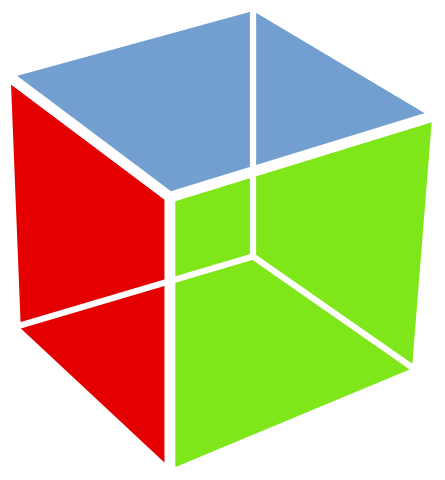
\includegraphics[width=\textwidth]{slides/graphics-software/gtk-logo.pdf}\\
  \vspace{3em}
  
\includegraphics[width=\textwidth]{slides/graphics-software/qt-logo.pdf}\\
  \vspace{3em}
  
\includegraphics[width=\textwidth]{slides/graphics-software/sdl-logo.png}\\
  \vspace{2em}
  \end{minipage}
  \hfill
  \begin{minipage}[b]{0.8\textwidth}
  \begin{itemize}
  \item Applications rarely to never use Wayland or X11 directly
  \item Drawing and managing a user interface is complex
  \item Widely-used high-level graphics libraries (aka toolkits)
    \begin{itemize}
    \item \textbf{GTK} (C): Widget-based UI toolkit, drawing helpers (GDK)
    \item \textbf{Qt} (C++): Widget-based UI toolkit, wide framework
    \item \textbf{EFL} (C): Lightweight UI and application library
    \item \textbf{SDL} (C): Drawing-oriented graphics library (used in games)
    \end{itemize}
  \item A desktop environment groups related libraries and components\\
  \textit{gives a consistent look and feel across the system}
  \item \textbf{Desktop environment} examples
    \begin{itemize}
    \item \textbf{GNOME}: Using GTK, GNOME-Shell desktop
    \item \textbf{KDE}: Using Qt, Plasma desktop
    \item \textbf{Xfce}: Using GTK, lightweight
    \item \textbf{Enlightenment}: Using EFL
    \end{itemize}
  \end{itemize}
  \vfill~
  \end{minipage}
  \begin{minipage}[b]{0.09\textwidth}
  \centering
  \includegraphics[width=\textwidth]{slides/graphics-software/gnome-logo.pdf}\\
  \vspace{1em}
  \includegraphics[width=\textwidth]{slides/graphics-software/kde-logo.pdf}\\
  \vspace{1em}
  \includegraphics[width=\textwidth]{slides/graphics-software/xfce-logo.pdf}\\
  \vspace{0.5em}
  \includegraphics[width=\textwidth]{slides/graphics-software/enlightenment-logo.pdf}
  \end{minipage}
\end{frame}

\subsection{TTY Kernel Aspects}

\begin{frame}{Linux TTY subsystem introduction}
  \begin{itemize}
  \item The \textbf{TTY} subsystem handles teletypewriters to send/receive characters
  \item Source code located at \code{drivers/tty} in Linux
  \item Supports physical instances (e.g. UART, RS-232) and virtual ones
  \item Virtual terminals/consoles (VTs/VCs) associate a distinct keyboard and display
    \begin{itemize}
    \item Many VTs are created by Linux, available under \code{/dev/tty*}
    \item Only a single VT is active at a time, switched with \code{Ctrl + Alt + Fi}
    \item Display grabbed using \textbf{fbcon} from the \textbf{fbdev} subsystem
    \item Keyboard grabbed using the \textbf{input} subsystem
    \item Can be used to show kernel messages (\code{console=tty1} in the cmdline)
    \item Every program runs under a controlling tty (given by the \code{tty} command)
    \end{itemize}
  \item Pseudo-terminals also exist, for software-based I/O only
    \begin{itemize}
    \item Created by programs (e.g. terminal emulator) under \code{/dev/pts/*}
    \item Unrelated to graphics topics
    \end{itemize}
  \end{itemize}
\end{frame}

\begin{frame}{Linux TTY (illustrated)}
  \begin{center}
    \includegraphics[width=0.6\textwidth]{slides/graphics-software/getty.jpg}\\
    \textit{Getty running on \code{tty1} of a GNU/Linux system}\\
  \end{center}
\end{frame}

\begin{frame}[fragile]{Virtual terminals and graphics}
  \begin{itemize}
  \item With VTs, the kernel is \textbf{already using} the display and keyboard!
  \item Display servers need to switch to \textbf{graphics mode} to release the display:
  \begin{minted}[fontsize=\small]{console}
ret = ioctl(tty_fd, KDSETMODE, KD_GRAPHICS);
  \end{minted}
  \item And disable \textbf{keyboard support} on the standard input:
  \begin{minted}[fontsize=\small]{console}
ret = ioctl(tty_fd, KDSKBMODE, K_OFF);
  \end{minted}
  \item The display device can then be used \textbf{exclusively}
  \item Input is no longer interpreted (e.g. \code{Ctrl-C} is ignored)
  \item Graphics and keyboard mode must be restored when leaving to keep the VT usable
  \item Current modes can be queried with:
  \begin{minted}[fontsize=\small]{console}
short mode, kbmode;
ret = ioctl(tty_fd, KDGETMODE, &mode);
ret = ioctl(tty_fd, KDGKBMODE, &kbmode);
  \end{minted}
  \item More details in the \code{console_ioctl} man page
  \end{itemize}
\end{frame}

\begin{frame}[fragile]{Virtual terminals switching and graphics}
  \begin{itemize}
  \item However, the user might still want to switch VTs!
  \item So the display device must be \textbf{released/reacquired} for VT switching
  \item UNIX signals are used to notify the application, configured with:
  \begin{minted}[fontsize=\small]{console}
struct vt_mode vt_mode = { 0 };
vt_mode.mode = VT_PROCESS;
vt_mode.relsig = SIGUSR1;
vt_mode.acqsig = SIGUSR2;
ret = ioctl(tty_fd, VT_SETMODE, &vt_mode);
  \end{minted}
  \item VT switching must be acknowledged for the other VT to take over:
  \begin{minted}[fontsize=\small]{console}
ret = ioctl(tty_fd, VT_RELDISP, VT_ACKACQ); /* when entering VT */
ret = ioctl(tty_fd, VT_RELDISP, 1); /* when leaving VT */
  \end{minted}
  \item Failure to acknowledge will cause a \textbf{system hang}
  \end{itemize}
\end{frame}

\subsection{Framebuffer Device Kernel Aspects}

\begin{frame}{Fbdev overview}
  \begin{itemize}
  \item Fbdev is the \textbf{historical and legacy} display subsystem in Linux
  \item Exposes a number of display-related features:
    \begin{itemize}
    \item Framebuffer access (pre-allocated for one or two frames)
    \item Operation primitives (bit blit, solid fill, area copy, etc)
    \item Cursor drawing
    \item Power management (blank/unblank, power down)
    \end{itemize}
  \item Initial state can be configured with the \code{video} option of the \code{cmdline}
  \item Available to userspace via \code{/dev/fb*} nodes:
    \begin{itemize}
    \item Generic base \code{ioctls} with driver-specific additions
    \item Direct framebuffer memory mapping using \code{mmap}
    \item Relatively simple and minimalistic interface
    \end{itemize}
  \item Used by the kernel to provide a graphical console with \textbf{fbcon}
  \end{itemize}
\end{frame}

\begin{frame}[fragile]{Fbdev basic operations}
  \begin{itemize}
  \item \textbf{Fixed information} about the display is retrieved with:
  \begin{minted}[fontsize=\small]{console}
struct fb_fix_screeninfo fix_screeninfo = { 0 };
ret = ioctl(fb_fd, FBIOGET_FSCREENINFO, &fix_screeninfo);
  \end{minted}
  \item \textbf{Variable information} (including mode) is retrieved and configured with:
  \begin{minted}[fontsize=\small]{console}
struct fb_var_screeninfo var_screeninfo = { 0 };
ret = ioctl(fb_fd, FBIOGET_VSCREENINFO, &var_screeninfo);
...
ret = ioctl(fb_fd, FBIOPUT_VSCREENINFO, &var_screeninfo);
  \end{minted}
  \item \textbf{Power management} is operated with:
  \begin{minted}[fontsize=\small]{console}
ret = ioctl(fb_fd, FBIOBLANK, FB_BLANK_POWERDOWN);
  \end{minted}
  \item \textbf{Double-buffering} is sometimes supported (within the same buffer):
  \begin{minted}[fontsize=\small]{console}
var_screeninfo.yoffset = height;
ret = ioctl(fb_fd, FBIOPAN_DISPLAY, &var_screeninfo);
  \end{minted}
  \item Blocking until the next \textbf{vblank} is possible with:
  \begin{minted}[fontsize=\small]{console}
int vsync = 0;
ret = ioctl(fb_fd, FBIO_WAITFORVSYNC, &vsync);
  \end{minted}
  \end{itemize}
\end{frame}

\begin{frame}{Fbdev limitations}
  \begin{itemize}
  \item Fbdev does not expose or allow configuration of the display pipeline
  \item Output setup is mostly static (provided through the \code{cmdline})
  \item Designed for simple cases (with a single output)
  \item Buffer allocation and management is not available
  \item No possibility of zero-copy import from other devices
  \item Limited page flipping with no associated synchronization mechanism
  \item Insufficient external synchronization interface (blocking wait)
  \item Mixes display, operation primitives and power management
  \end{itemize}

  \begin{center}
  \textbf{Fbdev is mostly adapted to display from the 1990s and 2000s}\\
  \small please consider avoiding it at all costs!
  \end{center}
\end{frame}

\subsection{DRM Kernel Aspects}

\begin{frame}{DRM devices}
  \begin{itemize}
  \item UNIX-style devices are identified with major/minor numbers
    \begin{itemize}
    \item More details in the \code{makedev} manpage, using \code{dev_t} type
    \item Minor/major can be retrieved with \code{stat/fstat}
    \item DRM major in Linux is \textbf{226}
    \end{itemize}
  \item Two types of DRM devices exist:
    \begin{itemize}
    \item \textbf{Primary} nodes at \code{/dev/dri/card*} with minor \(< 128\)\\
    Used for display operations with the KMS (mode) interface
    \item \textbf{Render} nodes at \code{/dev/dri/renderD*} with minor \(\geq 128\)\\
    Used for render operations with a driver-specific interface
    \end{itemize}
  \item DRM devices can also be used by the kernel directly (internal clients):
    \begin{itemize}
    \item \textbf{fbdev} compatibility layer to provide \code{/dev/fb*} nodes
    \item Used by \textbf{fbcon} to provide virtual consoles
    \end{itemize}
  \item Userspace needs rights to open device nodes:
    \begin{itemize}
    \item Usually allowed via the \code{video} \textbf{group} or \textbf{Access Control Lists} (ACLs)
    \end{itemize}
  \end{itemize}
\end{frame}

\begin{frame}[fragile]{DRM driver identification and capabilities}
  \begin{itemize}
  \item Driver-specific \textbf{name and version} (major/minor/patchlevel) can be queried:%
  \begin{minted}[fontsize=\small]{console}
struct drm_version version = { ... };
ret = ioctl(drm_fd, DRM_IOCTL_VERSION, &version);
  \end{minted}
  \item Drivers expose specific \textbf{capabilities}, that can be queried:
  \begin{minted}[fontsize=\small]{console}
struct drm_get_cap get_cap = { 0 };
get_cap.capability = DRM_CAP_DUMB_BUFFER;
ret = ioctl(drm_fd, DRM_IOCTL_GET_CAP, &get_cap);
  \end{minted}
  \item The kernel \textbf{must} be informed of client support for some features:
  \begin{minted}[fontsize=\small]{console}
struct drm_set_client_cap client_cap = { 0 };
client_cap.capability = DRM_CLIENT_CAP_UNIVERSAL_PLANES;
client_cap.value = 1;
ret = ioctl(drm_fd, DRM_IOCTL_SET_CLIENT_CAP, &client_cap);
  \end{minted}
  \item Driver and client capabilities defined in Linux's \kfile{include/uapi/drm/drm.h}
  \end{itemize}
\end{frame}

\begin{frame}[fragile]{DRM master, magic and authentication}
  \begin{itemize}
  \item Multiple userspace clients can open the same primary device node
  \item Only the \textbf{master} client is allowed to configure display (KMS)
  \item Master is exclusive and can be \textbf{acquired} and \textbf{dropped} (VT switching):
  \begin{minted}[fontsize=\small]{console}
ret = ioctl(drm_fd, DRM_IOCTL_SET_MASTER, NULL);
ret = ioctl(drm_fd, DRM_IOCTL_DROP_MASTER, NULL);
  \end{minted}
  \item Requires \code{CAP_SYS_ADMIN} Linux capability, see \code{capabilities} man page\\
    \textit{usually reserved to the root super user}
  \item Some operations can be allowed on trusted clients with \textbf{magic authentication}:
  \begin{enumerate}
  \item Client \textit{foo} gets its client-specific magic:
  \begin{minted}[fontsize=\small]{console}
struct drm_auth auth = { 0 };
ret = ioctl(drm_fd, DRM_IOCTL_GET_MAGIC, &auth);
  \end{minted}
  \item Client \textit{foo} sends \code{auth.magic} to master client \textit{bar} (via IPC)
  \item Master client \textit{bar} authenticates client \textit{foo}:
  \begin{minted}[fontsize=\small]{console}
ret = ioctl(drm_fd, DRM_IOCTL_AUTH_MAGIC, &auth);
  \end{minted}
  \end{enumerate}
  \item Mostly used before render nodes or for allocating buffers on another process
  \end{itemize}
\end{frame}

\begin{frame}[fragile]{DRM memory management}
  \begin{itemize}
  \item The \textbf{Graphics Execution Manager} (GEM) handles memory in DRM
  \item Used both by KMS and render drivers, with specific backends:
    \begin{itemize}
    \item \textbf{CMA}: Contiguous Memory Allocator (reserved area at boot)
    \item \textbf{Shmem}: Shared system memory (anonymous pages)
    \item \textbf{Vram}: Video RAM, using the \textbf{Translation Table Manager} (TTM)
    \end{itemize}
  \item Ensures buffers \textbf{coherency} on access (cache management)
  \item Allocated buffers are identified with a unique \textbf{handle} number
  \item In KMS, the \textbf{dumb buffer} API exposes memory operations:
    \begin{itemize}
    \item For memory used for \textbf{scanout framebuffers}
    \item Drivers calculate aligned pitch/stride and size based on dimensions and bpp
    \item Sometimes too limiting (e.g. multi-planar formats)
    \end{itemize}
  \item More details in the \textit{drm-memory} man page
  \item Drivers sometimes expose extra \code{ioctls} for more advanced needs
  \end{itemize}
\end{frame}

\begin{frame}[fragile]{DRM KMS dumb buffer API}
  \begin{itemize}
  \item \textbf{Allocating} from \code{width}, \code{height} and \code{bpp}, returning \code{handle}, \code{pitch} and \code{size}:\\
  \begin{minted}[fontsize=\small]{console}
struct drm_mode_create_dumb create_dumb = { ... };
ret = ioctl(drm_fd, DRM_IOCTL_MODE_CREATE_DUMB, &create_dumb);
  \end{minted}
  \item \textbf{Destroying} an allocated buffer:
  \begin{minted}[fontsize=\small]{console}
struct drm_mode_destroy_dumb destroy_dumb = { .handle = ..., };
ret = ioctl(drm_fd, DRM_IOCTL_MODE_DESTROY_DUMB, &destroy_dumb);
  \end{minted}
  \item \textbf{Preparing a mapping} in user memory for a buffer, returning an \code{offset}:
  \begin{minted}[fontsize=\small]{console}
struct drm_mode_map_dumb map_dumb = { .handle = ..., };
ret = ioctl(drm_fd, DRM_IOCTL_MODE_MAP_DUMB, &map_dumb);
  \end{minted}
  \item \textbf{Mapping memory} to userspace using the \code{offset}:
  \begin{minted}[fontsize=\small]{console}
map = mmap(NULL, create_dumb.size, PROT_READ | PROT_WRITE, MAP_SHARED,
           drm_fd, map_dumb.offset);
  \end{minted}
  \item \textbf{Unmapping} memory after use:
  \begin{minted}[fontsize=\small]{console}
munmap(map, create_dumb.size);
  \end{minted}
  \end{itemize}
\end{frame}

\begin{frame}[fragile]{DRM FourCCs and modifiers}
  \begin{itemize}
  \item DRM has its own representation of \textbf{pixel formats}, with FourCC codes (on 32 bits)
  \item Defined in the \kfile{include/uapi/drm/drm_fourcc.h} header
  \item They can specify up to 4 distinct \textbf{data planes} for color components
  \item Pixel formats are named "MSB-to-LSB" and specified in \textbf{little-endian} order\\
  \textit{LSB comes first in memory in little-endian}
  \item For instance, \code{DRM_FORMAT_XRGB8888} has the \code{B} byte first in memory\\
  \textit{Memory order is independent from the CPU or hardware endianness}
  \item A format \textbf{modifier} (on 64 bits) indicates the pixel order in memory
  \item \code{DRM_FORMAT_MOD_LINEAR} indicates raster order\\
  \textit{line-major left-to-right, top-to-bottom}
  \item Other modifiers are usually hardware-specific, often tiled\\
  (e.g. \code{DRM_FORMAT_MOD_VIVANTE_TILED})
  \end{itemize}
\end{frame}

\begin{frame}[fragile]{DRM KMS resources probing}
  \begin{itemize}
  \item KMS hardware resources are exposed through the following entities:
    \begin{itemize}
    \item Connectors
    \item Encoders
    \item CRTCs
    \item Planes: primary, overlay and cursor
    \item Framebuffers
    \end{itemize}
  \item Each resource instance is identified with a unique \textbf{identification number}
  \item The list of resource ids is retrieved with:
  \begin{minted}[fontsize=\small]{console}
struct drm_mode_card_res res = { ... };
ret = ioctl(drm_fd, DRM_IOCTL_MODE_GETRESOURCES, &res);
  \end{minted}
  \item Plane ids (that were introduced later) are retrieved with:
  \begin{minted}[fontsize=\small]{console}
struct drm_mode_get_plane_res res = { ... };
ret = ioctl(drm_fd, DRM_IOCTL_MODE_GETPLANERESOURCES, &res);
  \end{minted}
  \item Resource ids are used with subsequent resource-specific calls
  \end{itemize}
\end{frame}

\begin{frame}[fragile]{DRM KMS connector probing}
  \begin{itemize}
  \item The starting point to configure a KMS pipeline is the connector
  \item Current connector state is probed with:
  \begin{minted}[fontsize=\small]{console}
struct drm_mode_get_connector get_connector = { .connector_id = ... };
ret = ioctl(drm_fd, DRM_IOCTL_MODE_GETCONNECTOR, &get_connector);
  \end{minted}
  \item \code{struct drm_mode_get_connector} exposes various information:
    \begin{itemize}
    \item Connector type and connection state
    \item Possible encoders, currently-attached encoder
    \item Available modes and physical monitor size
    \end{itemize}
  \item Probing modes triggers EDID read: optional and usually quite slow
  \end{itemize}
\end{frame}

\begin{frame}[fragile]{DRM KMS modes}
  \begin{itemize}
  \item A display mode is represented as a \code{struct drm_mode_modeinfo} in DRM
  \item Members: \code{clock}, \code{[hv]display}, \code{[hv]sync_start}, \code{[hv]sync_end}, \code{[hv]total} and \code{flags} for signal-specific details (polarities)
  \item Diagram from \kfile{include/drm/drm_modes.h}:
  \begin{minted}[fontsize=\small]{console}
         Active                 Front           Sync           Back
         Region                 Porch                          Porch
<-----------------------><----------------><-------------><-------------->
  //////////////////////|
 ////////////////////// |
//////////////////////  |..................               ................
                                           _______________
<----- [hv]display ----->
<------------- [hv]sync_start ------------>
<--------------------- [hv]sync_end --------------------->
<-------------------------------- [hv]total ----------------------------->*
  \end{minted}
  \end{itemize}
\end{frame}

\begin{frame}[fragile]{DRM KMS encoder probing}
  \begin{itemize}
  \item The next step is to find which CRTC id can be used with the connector
  \item The encoder is the link between the connector and CRTC
  \item Current encoder state can be probed with:
  \begin{minted}[fontsize=\small]{console}
struct drm_mode_get_encoder get_encoder = { .encoder_id = ... };
ret = ioctl(drm_fd, DRM_IOCTL_MODE_GETENCODER, &get_encoder);
  \end{minted}
  \item \code{struct drm_mode_get_connector} exposes some information:
    \begin{itemize}
    \item Encoder type
    \item Possible CRTCs, currently-attached CRTC
    \end{itemize}
  \item This allows selecting the CRTC to use for the connector!
  \end{itemize}
\end{frame}

\begin{frame}[fragile]{DRM KMS framebuffer management}
  \begin{itemize}
  \item Framebuffers in DRM are described with a number of parameters :
    \begin{itemize}
    \item Picture-wide: \code{width}, \code{height}, \code{pixel_format}
    \item Plane-specific: GEM \code{handle}, \code{pitch}, \code{offset} and \code{modifier}
    \end{itemize}
  \item Up to 4 memory planes are supported (depending on the format)
  \item Allows supporting a wide range of possible configurations
  \item Flags are passed to indicate that modifiers or interlaced scan are used
  \item Framebuffers are registered from their parameters, returning a \code{fb_id}:
  \begin{minted}[fontsize=\small]{console}
struct drm_mode_fb_cmd2 fb_cmd2 = { ... };
ret = ioctl(drm_fd, DRM_IOCTL_MODE_ADDFB2, &fb_cmd2);
  \end{minted}
  \item They are destroyed using the \code{fb_id}:
  \begin{minted}[fontsize=\small]{console}
unsigned int fb_id = fb_cmd2.fb_id;
ret = ioctl(drm_fd, DRM_IOCTL_MODE_RMFB, &fb_id);
  \end{minted}
  \end{itemize}
\end{frame}

\begin{frame}[fragile]{DRM KMS CRTC configuration (legacy)}
  \begin{itemize}
  \item The pipeline can then be configured with the connector and the CRTC
  \item The current CRTC configuration can be retrieved with:
  \begin{minted}[fontsize=\small]{console}
struct drm_mode_crtc crtc = { .crtc_id = ... };
ret = ioctl(drm_fd, DRM_IOCTL_MODE_GETCRTC, &crtc);
  \end{minted}
  \item The CRTC is configured with the connector id
  \begin{minted}[fontsize=\small]{console}
struct drm_mode_crtc crtc = { .crtc_id = ... };
ret = ioctl(drm_fd, DRM_IOCTL_MODE_SETCRTC, &crtc);
  \end{minted}
  \item A mode and a framebuffer can be set (previous setup used otherwise)\\
  \textit{mandatory if the CRTC was unused before}
  \item The kernel will automatically select the best encoder for the connector and CRTC
  \item \textbf{Legacy and deprecated} way to do modesetting: only concerns the primary plane
  \end{itemize}
\end{frame}

\begin{frame}[fragile]{DRM KMS page flipping (legacy)}
  \begin{itemize}
  \item Page flipping is the action of switching the CRTC to another framebuffer\\
  \textit{only concerns the primary plane}
  \item An event can be requested when the flip happens
  \item Can be scheduled at different times (specified with \code{flags}):
    \begin{itemize}
    \item At a specified vblank target (absolute or relative) to avoid tearing
    \item As soon as possible (asynchronously) if supported
    \end{itemize}
  \begin{minted}[fontsize=\small]{console}
struct drm_mode_crtc_page_flip page_flip = { .crtc_id = ..., .fb_id = ... };
ret = ioctl(drm_fd, DRM_IOCTL_MODE_PAGE_FLIP, &page_flip);
  \end{minted}
  \item \textbf{Legacy and deprecated}: limited to the primary plane
  \end{itemize}
\end{frame}

\begin{frame}[fragile]{DRM KMS overlay plane configuration (legacy)}
  \begin{itemize}
  \item Overlay planes are configured separately from the CRTC main plane
  \item The current state of a plane can be retrieved with:
  \begin{minted}[fontsize=\small]{console}
struct drm_mode_get_plane get_plane = { .plane_id = ... };
ret = ioctl(drm_fd, DRM_IOCTL_MODE_GETPLANE, &get_plane);
  \end{minted}
  \item Provides possible CRTCs, current framebuffer and supported formats
  \item Planes are configured with source and destination parameters:
    \begin{itemize}
    \item \code{crtc_[xywh]}: On-CRTC position and dimensions
    \item \code{src_[xywh]}: In-framebuffer position and dimensions (source clipping area)
    \end{itemize}
  \item Configuration takes place with:
  \begin{minted}[fontsize=\small]{console}
struct drm_mode_set_plane set_plane = { .plane_id = ... };
ret = ioctl(drm_fd, DRM_IOCTL_MODE_SETPLANE, &set_plane);
  \end{minted}
  \item \textbf{Legacy and deprecated}: not synchronized to vblank or page flip
  \end{itemize}
\end{frame}

\begin{frame}[fragile]{DRM KMS cursor configuration and position (legacy)}
  \begin{itemize}
  \item Cursor planes have a separate dedicated legacy API
  \item Configured per-CRTC with a GEM \code{handle} and dimensions (\code{width}, \code{height})\\
  \textit{a zero GEM \code{handle} deconfigures and removes the cursor}
  \item Only supports the \code{DRM_FORMAT_ARGB8888} format (not configurable)
  \item Using a single \code{ioctl} with the \code{flags} field for the operation
  \begin{minted}[fontsize=\small]{console}
struct drm_mode_cursor cursor = { .flags = DRM_MODE_CURSOR_BO,
                                  .crtc_id = ...};
ret = ioctl(drm_fd, DRM_IOCTL_MODE_CURSOR, &cursor);
  \end{minted}
  \item Once configured, the cursor can be moved to \code{x}, \code{y} on-CRTC coordinates
  \begin{minted}[fontsize=\small]{console}
struct drm_mode_cursor cursor = { .flags = DRM_MODE_CURSOR_MOVE,
                                  .crtc_id = ... };
ret = ioctl(drm_fd, DRM_IOCTL_MODE_CURSOR, &cursor);
  \end{minted}
  \item \code{DRM_IOCTL_MODE_CURSOR2} variant provides cursor hotspot for virtual machines
  \end{itemize}
\end{frame}

\begin{frame}[fragile]{DRM event notification and wait}
  \begin{itemize}
  \item DRM provides an event notification mechanism for \textbf{vblank} and \textbf{page flip done}
  \item Available through the primary (KMS) file descriptor
  \item Can be used with \code{poll} and \code{select} (integrated in main loop)
  \item Events with a \code{struct drm_event} base are read using \code{read}
  \item Expand to \code{struct drm_event_vblank} for vblank and page flip done events\\
    \textit{only complete events are returned, so the buffer must be large enough}
  \item Events can be requested at page flip time or explicitly:
  \begin{minted}[fontsize=\small]{console}
union drm_wait_vblank wait_vblank = { .request = ... };
ret = ioctl(drm_fd, DRM_IOCTL_WAIT_VBLANK, &wait_vblank);
  \end{minted}
  \item A blocking wait for an absolute or relative vblank sequence can also be requested\\
  \textit{using the same \code{ioctl} and dedicated \code{request.type} values}
  \end{itemize}
\end{frame}

\begin{frame}[fragile]{DRM KMS object properties}
  \begin{itemize}
  \item KMS objects expose generic (or driver-specific) properties with names and values
  \textit{concerns \textbf{connectors}, \textbf{CRTCs} and \textbf{planes}}
    \begin{itemize}
    \item \textbf{Range} properties: limits for the value (signed or unsigned)
    \item \textbf{Enum} properties: fixed values with associated names for the values
    \item \textbf{Blob} properties: raw data with a given length
    \end{itemize}
  \item Properties have a \textbf{unique identifier across objects}, details can be queried:
  \begin{minted}[fontsize=\small]{console}
struct drm_mode_obj_get_property get_property = { .prop_id = ... }
ret = ioctl(drm_fd, DRM_IOCTL_MODE_GETPROPERTY, &get_property);
  \end{minted}
  \item Registered properties of an object can be retrieved using:
  \begin{minted}[fontsize=\small]{console}
struct drm_mode_obj_get_properties get_properties = { .obj_id = ... }
ret = ioctl(drm_fd, DRM_IOCTL_MODE_OBJ_GETPROPERTIES, &get_properties);
  \end{minted}
  \item The \code{value} of a property can be assigned with:
  \begin{minted}[fontsize=\small]{console}
struct drm_mode_obj_set_property set_property = { .obj_id = ..., .prop_id = ... }
ret = ioctl(drm_fd, DRM_IOCTL_MODE_OBJ_SETPROPERTY, &set_property);
  \end{minted}
  \item Blob properties need to be created and destroyed (with their own identifier)
  \end{itemize}
\end{frame}

\begin{frame}[fragile]{DRM KMS atomic}
  \begin{itemize}
  \item The legacy API comes with major design issues:
    \begin{itemize}
    \item Overlay and cursor plane updates are applied instantly (tearing)
    \item Plane updates cannot be synchronized together (intermediate states)
    \item No way to check that setup is valid before applying it
    \end{itemize}
  \item The atomic API lifts these restrictions with a new paradigm:
    \begin{itemize}
    \item Objects are configured based on their KMS properties\\
    \textit{values are affected to each changed property}
    \item Property changes of different objects are grouped in an \textbf{atomic commit}
    \item Planes are handled regardless of their type (primary, overlay, cursor)
    \item Commits can be marked for test only: checked but not applied
    \item Changes are applied at next vblank, unless marked asynchronous
    \end{itemize}
  \begin{minted}[fontsize=\small]{console}
struct drm_mode_atomic atomic = { ... }
ret = ioctl(drm_fd, DRM_IOCTL_MODE_ATOMIC, &atomic);
  \end{minted}
  \item Unless marked non-blocking, the \code{ioctl} returns when changes are applied
  \item A page flip event can also be requested
  \end{itemize}
\end{frame}

\begin{frame}[fragile]{DRM KMS atomic common properties}
  \begin{itemize}
  \item Common properties used to configure \textbf{connectors}:
    \begin{itemize}
    \item \code{CRTC_ID}: id of the CRTC to bind with the connector
    \end{itemize}
  \item Common properties used to configure \textbf{CRTCs}:
    \begin{itemize}
    \item \code{ACTIVE}: whether the CRTC is in use
    \item \code{MODE_ID}: id of the property blob with the \code{struct drm_mode_modeinfo} mode
    \end{itemize}
  \item Common properties used to configure \textbf{planes}:
    \begin{itemize}
    \item \code{FB_ID}: id of the framebuffer to bind with the plane
    \item \code{CRTC_ID}: id of the CRTC to bind with the plane
    \item \code{CRTC_[XYWH]}: on-CRTC position and dimensions of the plane
    \item \code{SRC_[XYWH]}: in-framebuffer position and dimensions (source clipping area)
    \end{itemize}
  \item Common properties used to probe \textbf{planes}:
    \begin{itemize}
    \item \code{TYPE}: type of the plane (primary/overlay/cursor)
    \item \code{IN_FORMATS}: list of supported formats/modifiers
    \end{itemize}
  \end{itemize}
\end{frame}

\begin{frame}[fragile]{DRM KMS atomic driver walkthrough}
  \begin{itemize}
  \item A state-of-the-art DRM KMS driver: \code{vc4} at \kdir{drivers/gpu/drm/vc4}\\
  \textit{integrates both DRM KMS and render}
  \item Entry point at \kfile{drivers/gpu/drm/vc4/vc4_drv.c}
  \item Dedicated documentation: \url{https://dri.freedesktop.org/docs/drm/gpu/vc4.html}
  \end{itemize}
\end{frame}

\begin{frame}[fragile]{DRM render generalities}
  \begin{itemize}
  \item DRM render drivers have their own \textbf{driver-specific API}\\
    \textit{unlike KMS, render hardware abstraction is done in userspace}
  \item Their API is exposed through custom \code{ioctls}
  \item Can be associated with a KMS driver (e.g. \code{vc4}) or separate (e.g. \code{v3d})
  \item Drivers handle memory, job submission and scheduling, interrupts
  \item DRM has a common scheduler (from AMD) in \kdir{drivers/gpu/drm/scheduler}
  \item Usual operations:
    \begin{itemize}
    \item Managing buffer objects (BOs) of different types (create, destroy, mmap)\\
    \textit{using GEM under the hood}
    \item Submitting job data structures for programming the GPU (command lists)\\
    \textit{with a validation step to ensure its validity}
    \item Waiting for operations to complete
    \item Exposing performance-related information
    \end{itemize}
  \end{itemize}
\end{frame}

\begin{frame}[fragile]{DRM render driver walkthrough}
  \begin{itemize}
  \item A state-of-the-art DRM render driver: \code{v3d} at \kdir{drivers/gpu/drm/v3d}
  \item Entry point at \kfile{drivers/gpu/drm/v3d/v3d_drv.c}
  \item Dedicated documentation: \url{https://dri.freedesktop.org/docs/drm/gpu/v3d.html}
  \end{itemize}
\end{frame}

\begin{frame}[fragile]{DRM Prime zero-copy memory sharing (dma-buf)}
  \begin{itemize}
  \item Memory buffers often need to be shared between different devices\\
    \textit{e.g. DRM KMS and DRM render but also concerns V4L2 for media devices}
  \item The kernel-wide \code{dma-buf} API allows exporting and importing buffers
  \item Buffers are represented as \textbf{file descriptors} in userspace\\
    \textit{file descriptors can be shared between programs via IPC}
  \item DRM exposes dma-buf via the \textbf{DRM Prime} API
  \item DRM prime exports a GEM \code{handle} to a returned \code{fd}:
  \begin{minted}[fontsize=\small]{console}
struct drm_prime_handle prime_handle = { .handle = ... }
ret = ioctl(drm_fd, DRM_IOCTL_PRIME_HANDLE_TO_FD, &prime_handle);
  \end{minted}
  \item And vice-versa:
  \begin{minted}[fontsize=\small]{console}
struct drm_prime_handle prime_handle = { .fd = ... }
ret = ioctl(drm_fd, DRM_IOCTL_PRIME_FD_TO_HANDLE, &prime_handle);
  \end{minted}
  \end{itemize}
\end{frame}

\begin{frame}[fragile]{DRM sync object fencing}
  \begin{itemize}
  \item In a multi-device pipeline with zero-copy, only scheduling is left to userspace\\
  \textit{each device signals completion and userspace moves on to the next}
  \item Fences were introduced to avoid the extra roundtrip in userspace:
    \begin{itemize}
    \item The flow of buffers between devices is usually known in advance
    \item The kernel can coordinate internally and trigger the next device
    \item Requires submitting all commands in advance with fences attached
    \end{itemize}
  \item DRM exposes fences via the \textbf{Sync object} API
  \item Sync objects contain one fence, exposed as a file descriptor
  \item The KMS atomic API and some render driver APIs take input fence fds
  \end{itemize}
\end{frame}

\begin{frame}[fragile]{DRM sync object fencing}
  \begin{itemize}
  \item Sync objects are created and destroyed with a \code{handle}:
  \begin{minted}[fontsize=\small]{console}
struct drm_syncobj_create syncobj_create = { 0 }
ret = ioctl(drm_fd, DRM_IOCTL_SYNCOBJ_CREATE, &syncobj_create);
  \end{minted}
  \begin{minted}[fontsize=\small]{console}
struct drm_syncobj_destroy syncobj_destroy = { .handle = syncobj_create.handle }
ret = ioctl(drm_fd, DRM_IOCTL_SYNCOBJ_DESTROY, &syncobj_destroy);
  \end{minted}
  \item An output fence's \code{fd} is exported from a device's sync object with:
  \begin{minted}[fontsize=\small]{console}
struct drm_syncobj_handle syncobj_handle = { .handle = handle, ... }
ret = ioctl(drm_fd, DRM_IOCTL_SYNCOBJ_HANDLE_TO_FD, &syncobj_handle);
  \end{minted}
  \item An input fence's \code{fd} is imported to a device's sync object with:
  \begin{minted}[fontsize=\small]{console}
struct drm_syncobj_handle syncobj_handle = { .handle = handle, .fd = fd }
ret = ioctl(drm_fd, DRM_IOCTL_SYNCOBJ_FD_TO_HANDLE, &syncobj_handle);
  \end{minted}
  \item Quite a recent feature, not yet available in V4L2 (media)
  \end{itemize}
\end{frame}

\begin{frame}[fragile]{DRM debug and documentation}
  \begin{itemize}
  \item \textbf{Debug message} using the \code{drm.debug} kernel cmdline argument:
    \begin{itemize}
    \item Detailed in the \kfile{include/drm/drm_print.h} header
    \item \code{drm.debug=0x17} for core, KMS, driver and atomic debug messages
    \end{itemize}
  \item Current \textbf{state debug} in debugfs: \code{cat /sys/kernel/debug/dri/0/state}
  \item Drivers expose \textbf{specific debugfs entries}
  \item \textbf{Debug utility}: \code{modetest} from \code{libdrm}
  \item \textbf{Community} contact:
    \begin{itemize}
    \item Mailing list: \code{dri-devel@lists.freedesktop.org}
    \item IRC channel: \code{#dri-devel} on the OFTC network
    \end{itemize}
  \item \textbf{Documentation} resources:
    \begin{itemize}
    \item Linux GPU Driver Developer’s Guide: \url{https://www.kernel.org/doc/html/latest/gpu/index.html}
    \item Man pages about userspace aspects: \code{drm}, \code{drm-kms}, \code{drm-memory}
    \end{itemize}
  \end{itemize}
\end{frame}

\subsection{DRM Userspace Aspects}

\begin{frame}{libdrm wrapper}
  \begin{itemize}
  \item Userspace access to DRM devices is wrapped with \textbf{libdrm}
  \item Exposes convenience wrappers, helpers and some data structures around \code{ioctls}
    \begin{itemize}
    \item For KMS support in the \code{libdrm.so} library
    \item For hardware-specific render drivers in dedicated libraries (e.g. \code{libdrm_nouveau.so})
    \end{itemize}
  \item Used by almost every userspace project dealing with DRM:\\
    \textit{weston, mutter, Xorg, mesa, etc}
  \end{itemize}

  \begin{center}
  \includegraphics[width=0.5\textwidth]{slides/graphics-software/libdrm-userspace.pdf}
  \end{center}
\end{frame}

\subsection{X Window Userspace Aspects}

\begin{frame}{X11 protocol and architecture}
  \begin{itemize}
  \item X11 core protocol implemented by Xorg:
    \begin{itemize}
    \item Asynchronous packet-based system with different types:\\
    \code{Request}, \code{Reply}, \code{Event} and \code{Error} packets
    \item Can be used locally (UNIX socket) or over network (TCP/IP)
    \end{itemize}
  \item Exposes \textbf{drawables} for clients to transfer or draw pixel data to the server:
    \begin{itemize}
    \item \textbf{Windows}: area of the display buffer owned by the application\\
      \textit{without backing storage, must be redrawn when occluded}
    \item \textbf{Pixmaps}: off-display backing storage that can be copied to windows
    \end{itemize}
  \item Windows are represented as a tree:
    \begin{itemize}
    \item Starting with the root window created by X
    \item Top-level windows and sub-windows created by clients
    \end{itemize}
  \item A graphics context (GC) allows requesting basic drawing and font rendering
  \item The server provides \textbf{input events} to concerned clients:
    \begin{itemize}
    \item Mouse movements relative to window coordinates
    \item Translated key symbols a from raw keycodes
    \end{itemize}
  \end{itemize}
\end{frame}

\begin{frame}{X11 protocol extensions}
  \begin{itemize}
  \item X11 has evolved over time through \textbf{extensions} to its main protocol
    \begin{itemize}
    \item Additional interfaces for X clients, matching \textbf{new hardware features}
    \end{itemize}
  \item \textbf{XKB}: complex keyboard layouts
  \item \textbf{Xinput2}: touchpad, touchscreen and multi-touch support
  \item \textbf{XSHM}: shared client/server memory, avoiding extra transfers/copies\\
    \textit{not\ possible to operate via the network}
  \item \textbf{XRandR}: monitor configuration and hotplugging without server restart
  \item \textbf{Composite}: delegates window composition to compositing window managers
  \item \textbf{XRender}: 2D rendering API with with alpha composition, rasterization, transformations, filtering
  \item \textbf{Xv}: video output format conversion and scaling offload in-DDX\\
    \textit{involves buffer copies and lacks synchronization with window position}
  \end{itemize}
\end{frame}

\begin{frame}{Xorg architecture and acceleration}
  \begin{itemize}
  \item Xorg is divided between generic and hardware-specific parts
  \item \textbf{Device-Independent-X} (DIX) concerns:
    \begin{itemize}
    \item X11 protocol implementation, client coordination
    \item Main event loop and event dispatching
    \item Graphics operations logic, boilerplate and fallback implementations
    \end{itemize}
  \item \textbf{Device-Dependent-X} (DDX) concerns:
    \begin{itemize}
    \item Input drivers (\code{xf86-input-...}) to grab events from the kernel
    \item Video drivers (\code{xf86-video-...}) to provide mode setting and 2D acceleration
    \end{itemize}
  \item \textbf{EXA} provides a 2D acceleration architecture between DIX and DDX
    \begin{itemize}
    \item Efficient way for drivers to expose accelerated 2D operation primitives
    \item Replaced the XFree86 Acceleration Architecture (XAA)
    \item Reduces driver boilerplate
    \end{itemize}
  \item \textbf{Glamor} provides 2D acceleration for the DDX using OpenGL 3D rendering
  \end{itemize}
\end{frame}

\begin{frame}{Xorg drivers overview}
  \begin{itemize}
  \item Generic Xorg \textbf{input} drivers:
    \begin{itemize}
    \item \code{xf86-input-libinput}: using \code{libinput} to get input events
    \item \code{xf86-input-evdev}: using the \code{evdev} kernel interface directly (\textbf{deprecated})
    \end{itemize}
  \item Specific Xorg \textbf{input} drivers:
    \begin{itemize}
    \item \code{xf86-input-synaptics}: for laptop touchpads
    \item \code{xf86-input-wacom}: for Wacom drawing tablets
    \item Specific drivers are \textbf{deprecated} in favor of \code{xf86-input-libinput}
    \end{itemize}
  \item Generic Xorg \textbf{display} drivers:
    \begin{itemize}
    \item \code{xf86-video-modesetting}: for \textbf{DRM KMS}, can be accelerated using \textbf{glamor}
    \item \code{xf86-video-fbdev}: for the \textbf{fbdev} interface, without acceleration (legacy)
    \item \code{xf86-video-vesa}: for the \textbf{Video BIOS Extension} (VBE) framebuffer (x86)
    \end{itemize}
  \item Specific Xorg \textbf{display} drivers:
    \begin{itemize}
    \item \code{xf86-video-[intel,nouveau,amdgpu]}: profiting from 2D acceleration blocks
    \item Specific drivers are deprecated in favor of \code{xf86-video-modesetting} and \textbf{glamor}\\
      \textit{the trend is to accelerate everything via 3D rendering instead of 2D accelerators}
    \end{itemize}
  \end{itemize}
\end{frame}

\begin{frame}{X11 and OpenGL acceleration: GLX and DRI2}
  \begin{itemize}
  \item Before DRM render nodes, there was a single device for KMS and render\\
    \textit{correlates with the idea of a graphics card mixing both aspects}
  \item The X server owns the graphics device \textbf{exclusively}
  \item Clients using OpenGL need to access the device for rendering
  \item The \textbf{GLX} API was introduced to perform \textbf{indirect rendering}:
    \begin{enumerate}
    \item Integrating OpenGL with the X Window API
    \item Forwarding GL calls to the GL implementation via the X server (AIGLX)\\
      \textit{introducing latency and performance issues}
    \end{enumerate}
  \item \textbf{The Direct Rendering Infrastructure} (DRI/DRI2) was introduced next:
    \begin{itemize}
    \item The X server authenticates DRI2 clients with DRM magic/auth\\
      \textit{allows them to access render features}
    \item Buffers are allocated by the X server and passed by references (\textit{GEM flinks})
    \item Rendering to buffers is done by the clients with the GL implementation
    \end{itemize}
  \item GLX is still used as a GL windowing API for X11
  \end{itemize}
\end{frame}

\begin{frame}{X11 and OpenGL acceleration: GLX and DRI2 (illustrated)}
  \begin{center}
  \includegraphics[width=0.4\textwidth]{slides/graphics-software/dri-data-flow.png}\\
  \textit{Data flow in X11 for different types of clients}
  \end{center}
\end{frame}

\begin{frame}{Xorg usage, integration and configuration}
  \begin{itemize}
  \item Xorg can be started with the \code{startx} command (wrapping \code{xinit})
    \begin{itemize}
    \item Executes server script from \code{/etc/X11/xinit/xserverrc} or \code{$HOME/.xserverrc}
    \item Executes client script from \code{/etc/X11/xinit/xinitrc} or \code{$HOME/.xinitrc}
    \end{itemize}
  \item An X \textbf{display manager} offers a login interface (e.g. KDM, LightDM)
    \begin{itemize}
    \item Runs under a Xorg server, with its own dedicated user
    \item Starts Xorg for authenticated users from session files in \code{/usr/share/xsessions/}
    \end{itemize}
  \item Used to require \textbf{running the server as root} to access graphics devices\\
    \textit{in particular, necessary to become DRM master}
    \begin{itemize}
    \item The \code{systemd-logind} login manager lifts the restriction
    \item Opens the DRM KMS fd privileged and passes it to Xorg via IPC
    \item Xorg can then drop privileges: details in the \code{Xorg.wrap} man page
    \end{itemize}
  \item Xorg is \textbf{configured} (both DIX and DDX) from \code{/etc/X11/xorg.conf}
  \item The \code{DISPLAY} environment variable indicates which server connection to use\\
    \begin{itemize}
    \item Already set for X client applications and inherited
    \item \code{export DISPLAY=:0} useful to launch programs from other TTYs
    \end{itemize}
  \end{itemize}
\end{frame}

\begin{frame}{Xorg architecture: input to display roundtrip}
  \begin{minipage}{0.49\textwidth}
    \centering
    \includegraphics[width=0.9\textwidth]{slides/graphics-software/x-architecture-roundtrip.png}
  \end{minipage}
  \hfill
  \begin{minipage}{0.49\textwidth}
    \begin{enumerate}
    \item An input event is read from the kernel by the server
    \item The affected client is determined and receives the event
    \item The client changes something and issues a rendering request
    \item The server performs rendering (DDX) and notifies the compositor
    \item The compositor updates the damaged regions in the back-buffer
    \item The server updates the display buffer from the compositor buffer (page flip)
    \end{enumerate}
  \end{minipage}
\end{frame}

\begin{frame}{Major issues with X11}
  \begin{itemize}
  \item The X11 core protocol and paradigm soon caused \textbf{various issues}:
    \begin{itemize}
    \item Based on buffer \textbf{copies, transfers} and frequent \textbf{redraws}\\
      \textit{solved with XSHM and DRI2 extensions}
    \item Immediate-mode drawing, with intermediate states scanned out\\
      \textit{solved by drawing everything client-side instead}
    \item Lack of synchronization/feedback interface\\
      \textit{specified with the DRI3 and Present extensions}
    \item Everything's a window with X... but not in practice (screensavers, popups)\\
    \textit{specified with the DRI3 and Present extensions}
    \item Heavy packet-based protocol causing \textbf{latency issues}
    \item \textbf{Security} concerns regarding client input/output isolation
    \end{itemize}
  \item Because the core protocol did not evolve, \textbf{extensions proliferated}:
    \begin{itemize}
    \item Complicated server aspects got \textbf{delegated} through extensions
    \item Working around major design issues, not solving them in depth
    \item In the end, the server mostly coordinates between other components
    \end{itemize}
  \item \textbf{Client-side rendering} became more common (raster, operations, fonts, etc)
  \end{itemize}
\end{frame}

\begin{frame}{Xorg code structure and walkthrough}
  \begin{itemize}
  \item Xorg source code available at: \url{https://gitlab.freedesktop.org/xorg/xserver}
  \item DDX components:
    \begin{itemize}
    \item Code specific to the Linux kernel under \code{hw/xfree86/os-support/linux/}
    \item Modesetting DRM KMS driver under: \code{hw/xfree86/drivers/modesetting/}
    \item fbdev core library under: \code{hw/xfree86/fbdevhw/}
    \item Glamor implementation under \code{glamor/}
    \end{itemize}
  \item DIX components:
    \begin{itemize}
    \item System-level helpers under \code{os/}
    \item Common framebuffer operations abstraction under \code{fb/}
    \item EXA abstraction under \code{exa/}
    \end{itemize}
  \item DRI2 components:
    \begin{itemize}
    \item DRI2 common code under \code{hw/xfree86/dri2}
    \item Modesetting DRI2 glue under \code{hw/xfree86/drivers/modesetting/dri2.c}
    \item GLX support under \code{glx/}
    \end{itemize}
  \end{itemize}
\end{frame}

\begin{frame}[fragile]{Xorg debug and documentation}
  \begin{itemize}
  \item Xorg has a \textbf{logging system} for all its components:
    \begin{itemize}
    \item Written to a file at \code{/var/log/Xorg.0.log}, \code{-logfile} option
    \item Verbosity can be set with the \code{-logverbose} option (log level)
    \item Printed on the standard output (\code{stdout})
    \end{itemize}
  \item Xorg can be bound to any VT with the \code{vt} command line option\\
    \textit{useful for remote debugging, with a virtual controlling terminal}
  \item \textbf{Community} contact:
    \begin{itemize}
    \item Mailing list: \code{xorg@lists.freedesktop.org}
    \item IRC channel: \code{#xorg} and \code{#xorg-devel} on the OFTC network
    \end{itemize}
  \item \textbf{Documentation} resources:
    \begin{itemize}
    \item Online wiki of the project: \url{https://www.x.org/wiki/Documentation/}
    \item Man pages: \code{X}, \code{Xserver}, \code{Xorg}, \code{xorg.conf}, \code{xinit} and more!
    \item Extensions specification documents
    \end{itemize}
  \end{itemize}
\end{frame}

\subsection{Wayland Userspace Aspects}

\subsubsection{Wayland}

\begin{frame}{Wayland overview and paradigm}
  \begin{itemize}
  \item Wayland was started in 2008 as a modern replacement for the X Window system\\
    \textit{solving issues in-depth with a clean implementation from scratch}
  \item Drastic \textbf{simplification} of the stack and paradigm shift:
    \begin{itemize}
    \item The server and compositor are \textbf{unified} as the same component
    \item \textbf{Clients} are expected to do all the rendering
    \item Buffers are \textbf{shared} between client and server, no transfers
    \item Window decorations can be added by the client or the server
    \end{itemize}
  \item Improves \textbf{security} aspects:
    \begin{itemize}
    \item Isolates the input and output of each client
    \item Only the compositor can access display buffers \textit{(and provide screenshots)}
    \item Avoids running the compositor as root (using \code{systemd-logind})
    \end{itemize}
  \item No network support (can be implemented by compositors)
  \item \textbf{Weston} is the reference \textbf{Wayland} compositor
  \end{itemize}
\end{frame}

\begin{frame}{Wayland architecture: input to display roundtrip}
  \begin{minipage}{0.49\textwidth}
    \centering
    \includegraphics[height=0.7\textheight]{slides/graphics-software/wayland-architecture-roundtrip.png}
  \end{minipage}
  \hfill
  \begin{minipage}{0.49\textwidth}
    \begin{enumerate}
    \item An input event is read from the kernel by the compositor
    \item The affected client is determined and receives the event
    \item The client changes something, performs rendering and notifies the compositor
    \item The compositor updates the damaged regions in the back-buffer and performs page flip
    \end{enumerate}
  \end{minipage}
\end{frame}

\begin{frame}{Wayland protocol and architecture}
  \begin{itemize}
  \item Wayland provides a client-server \textbf{low-level API}:
    \begin{itemize}
    \item Wayland \textbf{display connections} happen through local IPC
    \item Display is identified with the \code{WAYLAND_DISPLAY} \textbf{environment variable}
    \item \textbf{Asynchronous} and \textbf{object-oriented} protocol
    \item \textbf{Objects} represent \textbf{resources} from the compositor
    \item Objects implement specific \textbf{interfaces}, with requests and events
      \begin{itemize}
      \item \textbf{Requests} are messages sent by the client, 
      \item \textbf{Events} are messages received from the server\\
        \textit{errors are only specific types of events}
      \end{itemize}
    \end{itemize}
  \item Some \textbf{implementation} details:
    \begin{itemize}
    \item IPC is a regular UNIX socket (allows passing file descriptors for zero-copy)
    \item A proxy provides client-side object representations and message translation
    \item Messages are serialized (marshalling) to the wire format
    \item Messages are buffered and flushed/dispatched when asked
    \end{itemize}
  \item Client-server protocol is implemented in \textbf{libwayland-client} and \textbf{libwayland-server}
  \item These libraries do not provide any interface implementation
  \end{itemize}
\end{frame}

\begin{frame}{Wayland core protocol: global object interfaces}
  \begin{itemize}
  \item \textbf{Global} core object interfaces:
    \begin{itemize}
    \item \code{wl_display}: manages server connection, exposes the registry
    \item \code{wl_registry}: exposes available global object interfaces
    \item \code{wl_output}: describes the output properties (mode, geometry)
    \item \code{wl_seat}: exposes input device object capabilities and interfaces
    \item \code{wl_compositor}: provides surfaces and regions for composition
    \item \code{wl_subcompositor}: provides sub-surfaces for in-surface compositing
    \item \code{wl_shm}: exposes a shared memory interface
    \item \code{wl_data_device_manager}: support for copy/paste between clients
    \end{itemize}
  \item Global object interfaces are bound with the registry before use
    \begin{itemize}
    \item Using global \code{struct wl_interface} definitions
    \item \code{wl_registry_bind} returns a pointer to a proxy object
    \end{itemize}
  \item Global objects give access to other \textbf{specific objects}
  \end{itemize}
\end{frame}

\begin{frame}{Wayland core protocol: specific object interfaces}
  \begin{itemize}
  \item \textbf{Input-related} (\code{wl_seat}) specific core object interfaces:
    \begin{itemize}
    \item \code{wl_pointer}: exposes mice events and cursor
    \item \code{wl_keyboard}: exposes keyboard events and information
    \item \code{wl_touch}: exposes touchscreen events
    \end{itemize}
  \item \textbf{Compositor-related} (\code{wl_compositor}) specific core object interfaces:
    \begin{itemize}
    \item \code{wl_region}: specifies any area
    \item \code{wl_surface}: rectangular on-screen pixel area
      \begin{itemize}
      \item contents set to a \code{wl_buffer} (can be transformed)
      \item configured with a \code{wl_region} for input
      \item configured with a \code{wl_region} for area-based opacity
      \item updated with buffer damage regions
      \end{itemize}
    \item \code{wl_subsurface}: converts \code{wl_surface} objects to positioned sub-surfaces
    \end{itemize}
  \item \textbf{Shared memory-related} (\code{wl_shm}) specific core object interfaces:
    \begin{itemize}
    \item \code{wl_shm_pool}: allows creating shared-memory buffers
    \end{itemize}
  \item \textbf{Memory-related} specific core object interfaces:
    \begin{itemize}
    \item \code{wl_buffer}: generic object for a \code{wl_surface}
    \end{itemize}
  \end{itemize}
\end{frame}

\begin{frame}{Wayland extra protocols}
  \begin{itemize}
  \item Extra protocols (object interfaces) can be \textbf{exposed by the compositor}
    \begin{itemize}
    \item Protocols (including the core) are described as XML files
    \item The \code{wayland-scanner} tool produces client and server C code and headers
    \item Accepted additional protocol descriptions are available at:
      \url{https://gitlab.freedesktop.org/wayland/wayland-protocols}
    \item Some are considered stable and many unstable
    \end{itemize}
  \item Some widely-used \textbf{protocol extensions}:
    \begin{itemize}
    \item \textbf{XDG-Shell}: desktop shell integration
      \begin{itemize}
      \item Turns \code{wl_surfaces} to \code{xdg_surfaces} that can be resized, minimized, etc
      \item Provides a popup/menu interface with \code{xdg_popup}
      \end{itemize}
    \item \textbf{IVI-Shell}: In-vehicule shell with surface layers
    \item \textbf{Presentation time}: Precise timing and event feedback
    \end{itemize}
  \end{itemize}
\end{frame}

\begin{frame}{Wayland OpenGL integration}
  \begin{itemize}
    \item Wayland supports EGL for windowing integration with OpenGL
    \item \code{eglGetDisplay} is called with a \code{struct wl_display}\\
      \textit{mesa's \code{_eglNativePlatformDetectNativeDisplay} figures it out}
    \item Mesa 3D implements Wayland EGL interface for OpenGL integration
      \begin{itemize}
      \item Needs to implement DRI2 for DRM authentication
      \item \code{wl_drm} interface between the wayland EGL client and the compositor
      \item Both sides are actually implemented in mesa
      \item The interface is bound to the compositor with \code{eglBindWaylandDisplayWL}\\
        \textit{using the compositor's EGL context as entry-point to mesa}
      \item Allows sharing DRM GEM buffers with the compositor
      \end{itemize}
    \item Regular \code{wl_surfaces} can be bound to EGL:
      \begin{itemize}
      \item Converted to a \code{wl_egl_window} with \code{wl_egl_window_create}
      \item Then converted to an \code{EGLSurface} with \code{eglCreateWindowSurface}
      \end{itemize}
    \end{itemize}
\end{frame}

\begin{frame}{Wayland OpenGL integration (illustrated)}
  \begin{center}
  \includegraphics[width=12em]{slides/graphics-software/wayland-egl.pdf}\\
  \textit{\small Wayland integration with EGL}\\
  \end{center}
\end{frame}

\begin{frame}{Wayland status and adoption}
  \begin{itemize}
  \item Wayland is now quite mature, robust, efficient and widely used
    \begin{itemize}
    \item Most toolkits have support for it: GTK 3, Qt 5, SDL, EFL
    \item Major desktop environments support it: GNOME 3, KDE Plasma 5
    \item Integrated sessions with login managers from \code{/usr/share/wayland-sessions}
    \item Runs with user privileges with \code{systemd-logind}
    \end{itemize}
  \item X11 applications can be integrated using \textbf{XWayland}
    \begin{itemize}
    \item X server implementation registered as a Wayland client
    \item Wayland composer acts as X compositing window manager
    \item Creates a \code{wl_surface} for each window, redirects input/output
    \end{itemize}
  \item Diverse compositor implementations have emerged
    \begin{itemize}
    \item Sometimes tied to a desktop environment: mutter, kwin
    \item \textbf{libinput} was created to help with input aspects
    \item \textbf{libweston} emerged from the \textbf{Weston} compositor core
    \item \textbf{wlroots} emerged from the \textbf{Sway} compositor core
    \item Support \textbf{DRM KMS} display, \textbf{EGL} rendering (\textbf{pixman} supported by libweston)
    \end{itemize}
  \end{itemize}
\end{frame}

\begin{frame}{Wayland stack overview (illustrated)}
  \begin{center}
  \includegraphics[width=0.8\textwidth]{slides/graphics-software/wayland-stack.pdf}\\
  \textit{\small The graphics stack with Wayland}\\
  \end{center}
\end{frame}

\begin{frame}[fragile]{Wayland debug and documentation}
  \begin{itemize}
  \item \textbf{Debugging} tips:
    \begin{itemize}
    \item Supported global object interfaces can be listed with \code{weston-info}
    \item The \code{WAYLAND_DEBUG} environment variable enables protocol tracing
    \end{itemize}
  \item \textbf{Weston debugging}:
    \begin{itemize}
    \item Debug arguments: \code{--debug}, \code{--log=file.log}
    \item Grabbing a different TTY argument: \code{--tty 1}
    \item Wireframe keystroke: \code{mod + shift + space + F}
    \item Timeline recording (to a JSON file) keystroke: \code{mod + shift + space + d}\\
      \textit{can produce a graph with \url{https://github.com/ppaalanen/wesgr}}
    \end{itemize}
  \item \textbf{Community} contact:
    \begin{itemize}
    \item Mailing list: \code{wayland-devel@lists.freedesktop.org}
    \item IRC channel: \code{#wayland} on the OFTC network
    \end{itemize}
  \item \textbf{Documentation} resources:
    \begin{itemize}
    \item Online wiki of the project: \url{https://wayland.freedesktop.org/}
    \item Online documentation: \url{https://wayland.freedesktop.org/docs/html/}
    \end{itemize}
  \end{itemize}
\end{frame}

\subsection{Mesa 3D Userspace Aspects}

\begin{frame}[t]{Standardized 3D rendering APIs: OpenGL}
  \begin{center}
  \includegraphics[height=4em]{slides/graphics-software/opengl-logo.pdf}
  \end{center}

  \begin{itemize}
  \item 3D rendering API, designed for GPU \textbf{hardware acceleration}
    \begin{itemize}
    \item Generic API but \textbf{hardware-specific implementations}
    \item Started by \textbf{Silicon Graphics} in 1992, now managed by the \textbf{Khronos Group}
    \end{itemize}
  \item OpenGL provides a \textbf{high-level approach} to 3D graphics
    \begin{itemize}
    \item Compromise between complexity and fine-grained control
    \item Efficient abstraction, adapted to the hardware
    \item Leaves most memory management to the implementation
    \end{itemize}
  \item \textbf{Stateful} and \textbf{context-based} programming model
  \end{itemize}
\end{frame}

\begin{frame}[t]{Standardized 3D rendering APIs: OpenGL}
  \begin{center}
  \includegraphics[height=4em]{slides/graphics-software/opengl-logo.pdf}
  \end{center}

  \begin{itemize}
  \item OpenGL versions evolved with hardware features
    \begin{itemize}
    \item Version 1 targeted fixed-function pipeline GPUs
    \item Version 2 and up allow programming \textbf{vertex and fragment shaders}
    \item More shaders supported with new versions (\textit{geometry, tesselation})
    \end{itemize}
  \item OpenGL comes with the \textbf{GL Shading Language} (GLSL)
    \begin{itemize}
    \item Source code language for OpenGL shaders
    \item C-like syntax with intrinsic functions (e.g. texture access)
    \item Compiled on-the-fly by the GL implementation
    \end{itemize}
  \item Supports \textbf{extensions} that can be queried, for extra features
  \end{itemize}
\end{frame}

\begin{frame}[t]{Standardized 3D rendering APIs: OpenGL ES and EGL}
  \begin{minipage}[t]{0.49\textwidth}
    \centering
    \includegraphics[height=4em]{slides/graphics-software/opengl-es-logo.pdf}
  \end{minipage}
  \hfill
  \begin{minipage}[t]{0.49\textwidth}
    \centering
    \includegraphics[height=4em]{slides/graphics-software/egl-logo.pdf}
  \end{minipage}
  \vspace{0.5em}
  \begin{itemize}
  \item \textbf{OpenGL ES} was introduced as a simplified version for embedded devices
  \item OpenGL ES versions are loosely following OpenGL versions:
    \begin{itemize}
    \item Version 1 targets \textbf{fixed-function} GPUs
    \item Version 2 and up target \textbf{programmable} GPUs
    \end{itemize}
  \item Uses GLSL shaders and the same programming model as OpenGL
  \item \textbf{EGL} was introduced as standardized window integration API
    \begin{itemize}
    \item Connects with the native system display server
    \item Replaces GLX for X11 and adopted as default by Wayland
    \end{itemize}
  \item Supports \textbf{extensions} that can be queried, for extra platform-specific features
  \end{itemize}
\end{frame}

\begin{frame}[t]{Standardized 3D rendering APIs: Vulkan}
  \begin{center}
  \includegraphics[height=4em]{slides/graphics-software/vulkan-logo.pdf}
  \end{center}

  \begin{itemize}
  \item \textbf{Vulkan} is a \textbf{low-level} generic API for GPU access
    \begin{itemize}
    \item Started by the Khronos group in 2016 and widely adopted
    \end{itemize}
  \item Suitable for both \textbf{3D rendering} and \textbf{compute}
  \item Uses \textbf{Standard Portable Intermediate Representation} (SPIR-V) shaders
    \begin{itemize}
    \item Unified intermediate representation from (adapted) GLSL/HLSL sources
    \item Compiled with the program instead of on-the-fly (less overhead)
    \item Translated to native GPU operations by implementations
    \end{itemize}
  \item \textbf{Direct programming} model, with low-level \textbf{memory management}
  \item The API provides \textbf{window system integration} (WSI) for many platforms\\
    \textit{e.g. for Wayland: \code{vkCreateWaylandSurfaceKHR}}
  \end{itemize}
\end{frame}

\begin{frame}{Mesa 3D overview}
  \begin{itemize}
  \item Mesa is the reference free software \textbf{3D graphics implementation}
    \begin{itemize}
    \item Started back in 1993, evolved with GPU implementations
    \item Project works with the Khronos Group and develops extensions
    \end{itemize}
  \item Implements support for \textbf{rendering} APIs:
    \begin{itemize}
    \item \textbf{OpenGL} (up to 4.6) and \textbf{OpenGL ES} (up to 3.2)
    \item \textbf{Vulkan} (up to 1.1)
    \item \textbf{Direct 3D} (version 9 only)
    \end{itemize}
  \item Implements \textbf{windowing system} integration:
    \begin{itemize}
    \item \textbf{EGL} for Wayland, X11, Android, native DRM (GBM) and surface-less
    \item \textbf{Vulkan WSI} for Wayland and X11 (XCB/Xlib)
    \item \textbf{GLX} for X11
    \end{itemize}
  \item Also supports other \textbf{GPU-related features}:
    \begin{itemize}
    \item \textbf{Video decoding} acceleration via VDPAU, VAAPI, OMX
    \item \textbf{Compute} (GPGPU) support via OpenCL (\code{clover})
    \end{itemize}
  \end{itemize}
\end{frame}

\begin{frame}{Mesa 3D implementation highlights}
  \begin{itemize}
  \item Unlike other devices, 3D hardware is \textbf{abstracted in userspace}
    \begin{itemize}
    \item 3D rendering is a very bad fit for in-kernel abstraction
    \item Kernel drivers are much less complicated than GL implementations
    \end{itemize}
  \item Mesa implements driver-specific \textbf{DRM render} support\\
    \begin{itemize}
    \item Manages memory with the GEM and Prime DRM APIs
    \item Manages DRI2 to allow direct rendering
    \end{itemize}
  \item \textbf{Virtual} drivers are also supported (for virtual machines):
    \begin{itemize}
    \item \textbf{vmwgfx}: VMware bridge (proprietary virtual hardware implementation)
    \item \textbf{virgl}: Virtio bridge (standard for Linux and QEMU)
    \end{itemize}
  \item Also provides \textbf{software backends}:
    \begin{itemize}
    \item \textbf{softpipe}: Generic reference software renderer
    \item \textbf{swr}: OpenSWR renderer (for x86 by Intel)
    \item \textbf{llvmpipe}: LLVM-based renderer (high-performance)
    \end{itemize}
  \end{itemize}
\end{frame}

\begin{frame}{Mesa 3D internals: Gallium 3D}
  \begin{itemize}
  \item Classic mesa drivers have significant \textbf{code duplication}:
    \begin{itemize}
    \item API state tracking
    \item Compiler implementation
    \end{itemize}
  \item The Gallium 3D interface splits things up instead:
    \begin{itemize}
    \item \textbf{API State trackers}: maintain the current state for the API in use
    \item \textbf{Drivers}: implement shader compilation and hardware configuration
    \item \textbf{Winsys}: implement low-level kernel interfaces
    \end{itemize}
  \item Gallium drivers implement a pipe interface:
    \begin{itemize}
    \item \code{struct pipe_screen}: textures, buffers and sync management
    \item \code{struct pipe_state}: pipeline configuration and resources state
    \item \code{struct pipe_context}: rendering operation functions
    \end{itemize}
  \item Pipe loaders (DRM or software) select the right pipe driver
  \end{itemize}
\end{frame}

\begin{frame}{Mesa 3D internals: Gallium 3D (illustrated)}
  \begin{center}
  \includegraphics[width=0.5\textwidth]{slides/graphics-software/mesa-dri-gallium.pdf}\\
  \textit{\small Driver integration in Mesa 3D}
  \end{center}
\end{frame}

\begin{frame}{Mesa 3D internals: intermediate representations}
  \begin{itemize}
  \item Mesa is in charge of \textbf{compiling shaders} to the native shading ISA
  \item \textbf{Intermediate representations} (IRs) are used for translation
  \item \textbf{Input-level} IRs:
    \begin{itemize}
    \item \textbf{GLSL IR}: Internal GLSL shader representation
    \item \textbf{SPIR-V}: Khronos' Standard Portable Intermediate Representation
    \end{itemize}
  \item \textbf{Internal} IRs:
    \begin{itemize}
    \item \textbf{TGSI IR}: Tungsten Graphics Shader Interface representation
    \item \textbf{NIR}: New efficient internal representation for Mesa
    \item \textbf{Mesa}: Historical implementation (deprecated)
    \end{itemize}
  \item \textbf{External} IR:
    \begin{itemize}
    \item \textbf{LLVM IR}: Used for LLVM interaction (e.g. with llvmpipe)
    \end{itemize}
  \item Drivers emit \textbf{native instructions} from an internal IR and lowering
  \item Once ready, compiled shaders are \textbf{submitted to the GPU}
  \end{itemize}
\end{frame}

\begin{frame}{Mesa 3D internals: intermediate representations (illustrated)}
  \begin{center}
  \includegraphics[width=0.4\textwidth]{slides/graphics-software/mesa-ir.pdf}\\
  \textit{\small The Mesa 3D internal representation pipeline}
  \end{center}
\end{frame}

\begin{frame}[fragile]{Mesa 3D Generic Buffer Management}
  \begin{itemize}
  \item Mesa provides a Generic Buffer Management (GBM) interface:
    \begin{itemize}
    \item Buffer creation/destruction (supporting modifiers)
    \item Buffer information (bpp, dimensions, planes, stride, modifiers)
    \item Buffer mapping/unmapping
    \item Buffer dma-buf import/unimport
    \end{itemize}
  \item Compatible with the EGL API:
    \begin{itemize}
    \item \code{struct gbm_device} as \code{EGLNativeDisplayType}
    \item \code{struct gbm_surface} as \code{EGLNativeWindowType}
    \item \code{struct gbm_bo} as \code{EGLNativePixmapType}
    \end{itemize}
  \item Provided with DRM KMS fd for DRI2 (used internally for most operations)\\
  \begin{minted}[fontsize=\small]{console}
struct gbm_device *device = gbm_create_device(drm_fd);
  \end{minted}
  \item Useful when using bare-metal DRM KMS
  \end{itemize}
\end{frame}

\begin{frame}{Mesa 3D hardware support status: desktop}
  \begin{itemize}
  \item Updated Mesa per-driver support at \url{https://mesamatrix.net}
  \item \textbf{Intel HD/Iris Graphics}
    \begin{itemize}
    \item Platforms: Intel only
    \item Mesa driver: i965 (classic), iris (Gallium)
    \item DRM driver: i915
    \item Status: i965 is state-of-the art, iris in development
    \end{itemize}
  \item \textbf{Nvidia pre-NV110}
    \begin{itemize}
    \item Platforms: Tegra, any PCI-e compatible
    \item Mesa driver: nouveau (Gallium)
    \item DRM driver: nouveau
    \item Status: reverse engineered, advanced
    \end{itemize}
  \end{itemize}
\end{frame}

\begin{frame}{Mesa 3D hardware support status: desktop}
  \begin{itemize}
  \item \textbf{AMD Radeon GCN-ish}
    \begin{itemize}
    \item Platforms: AMD, any PCI-e compatible
    \item Mesa driver: radeonsi (Gallium)
    \item DRM driver: amdgpu
    \item Status: state-of-the art
    \end{itemize}
  \item \textbf{AMD Radeon R600+}
    \begin{itemize}
    \item Platform: AMD, any PCI-e compatible
    \item Driver: r600 (Gallium)
    \item DRM driver: radeon
    \item Status: advanced
    \end{itemize}
  \end{itemize}
\end{frame}

\begin{frame}{Mesa 3D hardware support status: embedded}
  \begin{itemize}
  \item \textbf{Qualcomm Adreno}
    \begin{itemize}
    \item Platforms: Qualcomm Snapdragon
    \item Mesa driver: freedreno (Gallium)
    \item DRM driver: freedreno
    \item Status: reverse engineered, advanced
    \end{itemize}
  \item \textbf{Vivante GCx000}
    \begin{itemize}
    \item Platforms: i.MX6, i.MX8, i.MX8M
    \item Driver: etnaviv (Gallium)
    \item DRM driver: etnaviv
    \item Status: work in progress, usable
    \end{itemize}
  \end{itemize}
\end{frame}

\begin{frame}{Mesa 3D hardware support status: embedded}
  \begin{itemize}
  \item \textbf{ARM Mali Utgard}
    \begin{itemize}
    \item Platforms: Exynos, Allwinner, Amlogic
    \item Mesa driver: lima (Gallium)
    \item DRM driver: lima
    \item Status: reverse engineered, early
    \end{itemize}
  \item \textbf{ARM Mali Midgard/Bifrost}
    \begin{itemize}
    \item Platforms: Rockchip, Exynos, Mediatek, Allwinner
    \item Mesa driver: panfrost (Gallium)
    \item DRM driver: panfrost
    \item Status: reverse engineered, early (but moving fast)
    \end{itemize}
  \end{itemize}
\end{frame}

\begin{frame}{Mesa 3D versus proprietary implementations}
  \begin{itemize}
  \item 3D support is one of the most challenging parts of hardware integration
  \item Proprietary implementations easily lead to various practical issues:
    \begin{itemize}
    \item Lack of support outside of prescribed environments
    \item Lack of specific features or APIs
    \item Lack of maintenance and updates
    \item No adaptation possibility
    \end{itemize}
  \item Mesa provides a collectively-maintained base
    \begin{itemize}
    \item Constantly updated and improved by the community
    \item Easier to manage: works out of the box with distributions
    \end{itemize}
  \item Mesa support is complex and often takes some time to bring performance\\
    \textit{especially for drivers based on reverse-engineering}
  \end{itemize}
\end{frame}

\begin{frame}{Mesa 3D code structure and walkthrough}
  \begin{itemize}
  \item Mesa source code available at: \url{https://gitlab.freedesktop.org/mesa/mesa}
  \item \textbf{Gallium 3D} components:
    \begin{itemize}
    \item Drivers under: \code{src/gallium/drivers/}
    \item Winsys under: \code{src/gallium/winsys/}
    \item API state trackers under: \code{src/gallium/state_trackers/}
    \item Pipe loaders under: \code{src/gallium/auxiliary/pipe-loader/}
    \end{itemize}
  \item \textbf{Compilation and IR} components:
    \begin{itemize}
    \item IR compiler support under \code{src/compiler/{glsl,nir,spirv}}
    \item TGSI support under \code{src/gallium/auxiliary/tgsi/}
    \item State tracking between IRs under \code{src/mesa/state_tracker}
    \end{itemize}
  \item \textbf{Windowing and DRI2} components:
    \begin{itemize}
    \item EGL support under \code{src/egl/drivers/dri2/}
    \item Vulkan WSI support under \code{src/vulkan/wsi/}
    \end{itemize}
  \item \textbf{Classic drivers} (DRI-1-style) under \code{src/mesa/drivers/dri/}
  \item \textbf{GBM} support under \code{src/gbm/}
  \end{itemize}
\end{frame}

\begin{frame}[fragile]{Mesa 3D hardware support: debug and documentation}
  \begin{itemize}
  \item Mesa is debugged with numerous \textbf{environment variables}
    \begin{itemize}
    \item Generic and per-driver, see \url{https://www.mesa3d.org/envvars.html}
    \item Shader-related, see \url{https://www.mesa3d.org/shading.html}
    \item \code{LIBGL_DEBUG=verbose} for OpenGL, \code{EGL_LOG_LEVEL=debug} for EGL
    \end{itemize}
  \item \code{eglinfo} and \code{glxinfo} show information about the implementation
  \item \textbf{Community} contact:
    \begin{itemize}
    \item Mailing list: \code{dri-devel@lists.freedesktop.org}
    \item IRC channel: \code{#dri-devel} on the OFTC network
    \end{itemize}
  \item \textbf{Documentation} resources:
    \begin{itemize}
    \item Online website: \url{https://www.mesa3d.org/}
    \item Gallium 3D wiki: \url{https://www.freedesktop.org/wiki/Software/gallium/}
    \item Gallium 3D documentation: \url{https://gallium.readthedocs.io/}
    \item Source code reference: \url{https://elixir.bootlin.com/mesa/latest/source}
    \end{itemize}
  \end{itemize}
\end{frame}

\begin{frame}{Graphics software online references}
  \small
  \begin{minipage}[t]{0.45\textwidth}
  \begin{itemize}
  \item Linux man pages
  \item Wikipedia (\url{https://en.wikipedia.org/}):
    \begin{itemize}
    \item \href{https://en.wikipedia.org/wiki/X_Window_System}{X Window System}
    \item \href{https://en.wikipedia.org/wiki/X.Org_Server}{X.Org Server}
    \item \href{https://en.wikipedia.org/wiki/Wayland_(display_server_protocol)}{Wayland (display server protocol)}
    \item \href{https://en.wikipedia.org/wiki/Mesa_(computer_graphics)}{Mesa (computer graphics)}
    \item \href{https://en.wikipedia.org/wiki/OpenGL}{OpenGL}
    \item \href{https://en.wikipedia.org/wiki/Vulkan_(API)}{Vulkan (API)}
    \end{itemize}
  \end{itemize}
  \end{minipage}
  \hfill
  \begin{minipage}[t]{0.5\textwidth}
  \begin{itemize}
  \item Freedesktop.org (\url{https://freedesktop.org/}):
    \begin{itemize}
    \item \href{https://dri.freedesktop.org/wiki/}{Direct Rendering Infrastructure}
    \item \href{https://dri.freedesktop.org/wiki/DRM/}{DRM}
    \item \href{https://wayland.freedesktop.org/}{Wayland}
    \item \href{https://www.x.org/wiki/}{X.org wiki}
    \end{itemize}
  \item Khronos (\url{https://khronos.org/}):
    \begin{itemize}
    \item \href{https://www.khronos.org/opengl/}{OpenGL}
    \item \href{https://www.khronos.org/opengl/wiki/}{OpenGL Wiki}
    \item \href{https://www.khronos.org/egl/}{EGL}
    \item \href{https://www.khronos.org/vulkan/}{Vulkan}
    \end{itemize}
  \end{itemize}
  \end{minipage}
\end{frame}

\begin{frame}{Graphics software illustrations attributions}
  \small
  \begin{itemize}
  \item \href{https://commons.wikimedia.org/wiki/File:X11.svg}{X11 logo: public domain}
  \item \href{https://commons.wikimedia.org/wiki/File:Wayland_Logo.svg}{Wayland logo: Kristian Høgsberg}
  \item \href{https://commons.wikimedia.org/wiki/File:GTK_logo.svg}{GTK logo: Andreas Nilsson, CC BY-SA 3.0}
  \item \href{https://commons.wikimedia.org/wiki/File:GTK_logo.svg}{Qt logo: Qt Project, public domain}
  \item \href{https://commons.wikimedia.org/wiki/File:SDL_Logo.svg}{SDL logo: Arne Claus / SDL Project, public domain}
  \item \href{https://commons.wikimedia.org/wiki/File:Gnomelogo.svg}{GNOME logo: GNOME Foundation, GNU LGPL 2.1+}
  \item \href{https://commons.wikimedia.org/wiki/File:KDE_logo.svg}{KDE logo: KDE e.V., GNU LGPL 2.1+}
  \item \href{https://commons.wikimedia.org/wiki/File:Xfce_logo.svg}{XFCE logo: Xfce Team, GNU LGPL 2.1+}
  \item \href{https://commons.wikimedia.org/wiki/File:Enlightenment_logo_black.png}{Enlightenment logo: Carsten Haitzler and various contributors, BSD}
  \end{itemize}
\end{frame}

\begin{frame}{Graphics software illustrations attributions}
  \small
  \begin{itemize}
  \item \href{https://commons.wikimedia.org/wiki/File:Devuan_GNU-Linux_-_tty_login_-_server_rack.jpg}{Devuan GNU-Linux - tty login - server rack: Francesco Magno, CC BY-SA 4.0}
  \item \href{https://commons.wikimedia.org/wiki/File:DRM_architecture.svg}{DRM architecture: Javier Cantero CC BY-SA 4.0}
  \item \href{https://wayland.freedesktop.org/architecture.html}{Wayland architecture: Wayland Developers, GNU GPL 2+}
  \item \href{https://wayland.freedesktop.org/architecture.html}{X architecture: Wayland Developers, GNU GPL 2+}
  \item \href{https://commons.wikimedia.org/wiki/File:Wayland_display_server_protocol.svg}{Wayland display server protocol: Shmuel Csaba Otto Traian, CC BY-SA 3.0}
  \item \href{https://commons.wikimedia.org/wiki/File:The_Linux_Graphics_Stack_and_glamor.svg}{The Linux Graphics Stack and glamor: Shmuel Csaba Otto Traian, CC BY-SA 3.0}
  \item \href{https://www.khronos.org/assets/utilities/retrieveFile.php?d=opengl&t=logopacks}{Khronos logo pack}
  \item \href{https://commons.wikimedia.org/wiki/File:Gallium3D_vs_DRI_graphics_driver_model.svg}{Gallium3D vs DRI graphics driver model, CC BY-SA 3.0}
  \end{itemize}
\end{frame}
